\chapter{绪论}
水声传感器网络(Under-water Acoustic Sensor Networks, UW-ASNs)指的是在一定的水下区域内,通过各种传感器获取信息,并对水下节点进行水声通信和组网,进而实现信息的传输目的/cite{Underwater acoustic sensor networks}。UW-ASNs可用于检测和采集数据,也会为水下航行器的导航提供支持,例如识别海底礁石和水下定位。


\section{研究背景}
UW-ASNs由多个水下固定传感器节点和移动节点如UUV和AUV等组成,这些节点被布放在水下一个给定区域内,共同执行观测任务。下图是一个典型的水声传感器网络,AUV、固定结点和海面浮标之间可以相互通信,海面浮标和控制中心利用卫星通信。
\begin{figure}[ht]
	\centering
	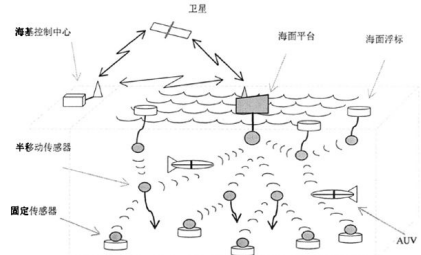
\includegraphics[scale=0.8]{figures/1.png}
	\caption{
		水声传感网络
	}
	\label{fig:example}
\end{figure}

搭载有各种设备的AUV可以在水下按特定轨迹航行,是水下传感网络中常用的移动平台。AUV的加入为海洋立体观测提供了可能,扩大了网络的监控范围;同时AUV可以对网络进行配置,如节点失效时,AUV可以检测通信空洞并指导布放新节点,提高网络的稳健性。

\subsection{水声传感网络结构}
开放系统互联协议栈模型(0sI,0penSystemsIntercollnection),OsI是有7层组成的,也是划分最细的一个。不同于OSI,水声传感器网络协议栈(UWASN,Unden) ̄raterAcousticSensorNe帆ork)是由三个层次组成的。这三个层次从下到上分别为物理层、数据链路以及网络层。由此可见,它的架构也不同于传输控制/网际通讯协议(TCP/IP,
TraIIsmission Con仃ol Protocol/IntemetProtoc01),TCP/IP是由5个部分组成的。

\subsection{水声传感网络国内外现状}
1993年,在美国海军研究办公室(ONR)资助的自治海洋采集网络(AOSNs)中
最早提出了水声通信网络应用的概念,该项目试图通过建立一个以AUV做为移动节点
的智能海洋数据采集网络来收集海洋数据,并于2003年在蒙特利海湾(Monterey Bay)
成功进行了海试。
1994年,美国伍兹霍尔海洋研究所(WHOI)开发了第一代水声通信局域网(AIA蛳,
该网络由一个海面浮标站和十几个1000m水深的海底节点构成,主要功能是将海底节点
产生的数据发往水面站以及将水面站产生的控制信息发向海底节点。
1996年美国在墨西哥湾进行了TBED(telemetry buoy
environmental data)96试验。
该试验是海网(Scaweb)试验的前身,在试验中使用了第一代商业化的基于DSP技术
的Tclesonar(具有远程通信能力的声纳)调制解调器Datasonics ATM850。该调制解调
器工作方式为MFSK,媒体接入方式为TDMA。TBED是第一个无中心结构的水声通信
数字网络,网络节点容量最多可达10个。无中心结构是海网(Scaweb)的重要特征。
TBED网络中的节点采用广播中继方式进行数据交互,最终达到网关节点。
为了研究基于水声通信的无线组网技术,美国分别于1998、1999、2000
欧共体在MAST计划的支持下开展了一系列的水声通信网络研究,主要包括
ACME,LOTUS、SWAN、ROBLINKS等子计划。其中ACME是研究基于浅水网络的
稳健通信和网络协议,网络中节点最小数为3,水深6.10米,节点之间的距离是200.2000
米,最高数据率是lkbit/s。LOTUS主要是研究基于超浅水域的长距离通信设备,其中
点对点之间的通信距离可达到10km,载波频率为8kHz,最高数据速率4kbit/s,该系统
针对超浅水域中存在的强时变的混响干扰以及多用户干扰等问题进行了技术攻关。使用
三维水听器阵列进行空间分集,同时对每~个发送端进行匹配,目前该系统已经进行了
两次海上试验。SWAN计划的目标是在浅海条件下建立通信仿真模型.研究各种无训练
条件下MEMU阵列处理方法。ROBLINKS计划主要是研究浅海条件下,水深20m--一30m,
距离大于10km的稳健通信项目,开发新的最佳相关信号处理算法是其研究重点,通过
连续信道辨识技术,提高通信系统对周围环境变化的适应能力,并对算法进行海上验证
130l。
目前国内对于水声通信网的研究还处于起步阶段,还没有进行过大规模的海上试
验,仅停留在理论仿真研究上。主要研究机构有哈尔滨工程大学、东南大学、厦门大学、
中科院声学所、中国海洋大学、西北工业大学、华中科技大学等。研究内容主要是低速
率远程通信和高速率近程通信,以及一些组建通信网络的网络协议llSll2al。
\subsection{面临的问题}
1)代价:随着科技以及研究的深入和进步,陆地无线传感器网络如预期一样,价格越来越低的传感器节点,导致部署花费越来越少。而相对而言,还很的昂贵的水声传感器网络的硬件,目前来看,导致部署水声传感器网络的代价是非常大的。这是由于水声传感器网络的节点需要特制的收发器。需要大量的实验来设计一个适用于水下的收发器,并且为了让该收发器适用于水下恶劣的环境,如压强,温度等,也需要设计保护收发器的装置。这点来看,基本硬件就需要很大的代价。
(2)部署:相对于陆地无线传感器网络的密集部署的特点,水声传感器网络节点的密度相对来说要稀疏的多。首先部署水声传感器网络本身就具有巨大的难度,其次(1)中所说的代价也是个问题。
(3)能量:水声传感器网络所需要的能量远远高于陆地无线电传感器网络消耗的能量。节点之间相对更远的距离,以及为了弥补信道损耗,接收器对信号做了更复杂的处理都大大增加了能量的消耗。
(4)存储:由于水下环境的恶劣导致水声传感器网络间歇性的工作,这就要求水声传感器网络的节点需要有相对于陆地传感器网络较大的存储空间,以便当传感器节点无法连接网络时,有足大的空间存储数据。



\section{研究内容}
本研究针对有移动节点接入和水下固定传感器组成的小规模单跳网络,结合海洋信息采集中对移动水声传感网络的各类需求,从设计移动节点接入机制、降低整体传输时延等方面入手,进行了如下的研究:
\begin{itemize}
	\item 针对少量移动节点接入固定节点网络,单向采集固定节点数据的场景,设计移动节点的接入和离开机制。移动节点加入固定节点网络时,需要发送广播包通知固定节点进行数据传输,充分利用广播包特点,降低移动节点接入离开机制的开销,是流程设计时的重点。
	\item 当移动节点数量增加时,固定节点传输的目标节点的选择会影响整体网络的性能。在选择目标节点时,一要考虑目标节点与固定节点的远近,这会影响到数据的传输时延;二要考虑目标节点的负载情况,使网络负载相对均衡。因此固定节点要根据实时的网络情况,自适应得进行最优目标节点的选择。
	\item 考虑到水声环境的特殊性,基于RTS/CTS握手机制的竞争协议应用在水声信道中需要进行协议流程和参数的进一步优化。
\end{itemize}

\section{章节安排}
本文的章节安排如下,

第一章绪论,主要介绍了水声传感网络的概念、发展历史和特点,说明了本文的研究背景和应用场景,在此基础上引出了研究的主要内容。

第二章分析了移动水声网络MAC协议研究的国内外现状。

第三章重点介绍了两个竞争型水声传感网络MAC协议,UWALOHA和SFAMA。

第四章针对有移动节点接入的单跳水声网络,提出了基于竞争的MAPA-CSMA协议。本章详细介绍了协议的流程设计和参数选择。其中,重点介绍了移动节点的接入离开机制和不同网络负载情况下的数据发送机制。

第五章针对提出的MAPA-CSMA协议进行理论计算。

第六章介绍了仿真的工具NS2,并且分析了仿真的结果。

\endinput